\documentclass[12pt]{article}
 
\usepackage[utf8x]{inputenc}
\usepackage[brazilian]{babel}
\usepackage{fontenc}
\usepackage{graphicx} 
\usepackage{listings}
\usepackage{xcolor}
\usepackage{indentfirst}
\usepackage{pdflscape}
\usepackage[bottom=3cm,top=3cm,left=3cm,right=3cm]{geometry} 
\usepackage[pdftex]{hyperref} %permitir \url

\usepackage{wallpaper}
\usepackage{subfig}

\usepackage{fancyhdr}
\pagestyle{fancy}
\fancyhf{}
\rhead{QXCode}
\lhead{Blackjack}
\fancyfoot[R]{\thepage}
%\rfoot{Page \thepage}


\usepackage[absolute]{textpos}


\lstset{
    language=java,
%    language=c++,
    keywordstyle=\bfseries\ttfamily\color[rgb]{0,0,1},
    identifierstyle=\ttfamily,
    commentstyle=\color[rgb]{0.133,0.545,0.133},
    stringstyle=\ttfamily\color[rgb]{0.627,0.126,0.941},
    showstringspaces=false,
    basicstyle=\small,
    tabsize=2,
    breaklines=true,
    frame=single
}



\renewcommand{\tt}[1]{\lstinline|#1|}
\renewcommand{\bf}[1]{\textbf{#1}}


\begin{document}

\ThisULCornerWallPaper{1}{./imagens/header}

\begin{textblock}{15}(0.4, 0.4)
\noindent
\begin{center}
\LARGE{\bf{QXCode - Quixadá Coding Team}}\\
\large{\bf{Fundamentos de Programação}} \\
\large{\bf{\today}}
\end{center}
\end{textblock}

\title{\bf{Blackjack \\ Um Jogo de Cartas Inocente}}

\author{
David Sena \thanks{sena.ufc@gmail.com}, 
Ronildo Oliveira. \thanks{ro.nildooliveira@hotmail.com}
}

\date{}

\maketitle
\thispagestyle{empty}

%#################################################################
%#################################################################
%#################################################################
%#################################################################


\section{Instruções Gerais}
O objetivo desse trabalho é simular o jogo de Blackjack 21 entre um usuário e a mesa. As opções do jogador são simplificadas em relação ao jogo original. 

%A sequencia da figura \ref{fig:blackjack} ganha o jogo.

\begin{figure}[hf]
\centering
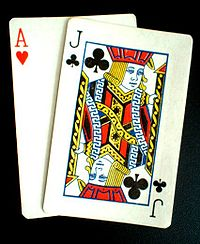
\includegraphics[width=0.3\linewidth]{./imagens/blackjack}
\caption{Ganhou}
%\label{fig:blackjack}
\end{figure}

\url{http://pt.blackjack.org/regras/}

\url{http://pt.wikipedia.org/wiki/Blackjack}

Você pode jogar online uma simulação bem parecida com a que vamos implementar para compreender as regras.

\url{http://jogosonline.uol.com.br/blackjack-gentleman-s-bet_43651.html}

\subsection{Regras Básicas}

Todas as cartas com 10 ou menos (2, 3, 4, 5, 6, 7 ,8, 9, 10) têm um valor igual a seu número. Os naipes não influenciam o valor das cartas (o quatro de paus possui o mesmo valor que o quatro de ouros). Por exemplo: se um jogador receber as seguintes cartas: 2, 5 e 8, o valor de todas as três equivalerá a 15.

Os valetes, damas e reis são todos equivalentes a 10. Como as cartas numeradas, naipes diferentes não afetam o valor dessas cartas. Por exemplo: se um jogador receber um valete ou um rei como suas duas primeiras cartas viradas para cima, elas equivalerão a 20, a segunda pontuação mais alta, abaixo apenas do 21.

A última carta, o ás, tem um valor especial no jogo de blackjack. O ás pode valer \bf{1} ou \bf{11}, com o número real dependente do valor mais vantajoso em uma mão específica. Um ás com um rei, rainha ou valete significa 21 pontos e o jogador ganha imediatamente. Se o valor da soma não ultrapassar 21, faça o ás valer 11. Se ultrapassar, vá transformando os Ás em 1 tentando baixar a soma.

\section{Implementação}
Opções do usuário : Pedir Carta (Hit) ou Parar.

O jogador inicia com 2 cartas e a mesa com 1 carta.

O jogador pode pedir quantas cartas quiser até parar
ou estourar o valor de 21.

Se o jogador parar sem estourar, a mesa vai jogar até
vencer o jogador ou estourar. Se a mesa tiver a mesma
quantidade de pontos do jogador ela vence.

Nos trechos que representam a saída do terminal, os símbolos \verb|>>| representam que o programa para e espera a entrada do usuário.

\subsection{Exemplo}

Uma única rodada, um jogador e a mesa. A cada rodada o programa pergunta se o jogador quer para ou continuar. Se quiser continuar, recebe uma carta aleatória. Abaixo, um exemplo de saída.

\begin{verbatim}
Iniciando Rodada:
# Mesa recebe  7 - Total  7 [ 7 ]
# Voce recebe  A - Total 11 [ A ]
# Voce recebe  2 - Total 13 [ A 2 ]
Pedir = 1, Parar = 2 
>> 1

# Voce recebe  3 - Total 16 [ A 2 3 ]
Pedir = 1, Parar = 2 
>> 2

# Mesa recebe  2 - Total  9 [ 7 2 ]
# Mesa recebe  7 - Total 16 [ 7 2 7 ]
# Mesa (16), Voce (16)
Voce perdeu!
\end{verbatim}

Nova execução do programa.

\begin{verbatim}
Iniciando Rodada:
# Mesa recebe  7 - Total  7 [ 7 ]
# Voce recebe  A - Total 11 [ A ]
# Voce recebe  2 - Total 13 [ A 2 ]
Pedir = 1, Parar = 2 
>> 1

# Voce recebe  Q - Total 13 [ A 2 Q ]
Pedir = 1, Parar = 2 
>> 1

# Voce recebe  5 - Total 18 [ A 2 Q 5 ]
Pedir = 1, Parar = 2 
>> 2

# Mesa recebe  8 - Total 15 [ 7 8 ]
# Mesa recebe  7 - Total 22 [ 7 8 7 ]

# Mesa (22), Voce (18)
Voce Ganhou
\end{verbatim}

\section{Melhorias}
\begin{itemize}

\item Você pode colocar um sistema de apostas, onde o jogador começa com uma certa quantidade de dinheiro e pode ganhar ou perder dinheiro.

\item Você pode manter o jogador jogando enquanto ele quiser ou tiver dinheiro.

\item Se você ainda quer um desafio, que tal implementar
um jogo para múltiplos jogadores? Pesquise um pouco sobre as regras para múltiplos jogadores.

\item Uma outra possibilidade é adicionar as regras
adicionais como dobrar ou partir as cartas.


\end{itemize}

Bom Trabalho.

\end{document}
